 
The Large Hadron Collider (LHC) is a proton-proton storage ring operating at CERN, and for its 9 years of operation, it has been the world's highest energy particle collider. 
%The LHC first began operation in 2008 but following a magnetic quench incident it had to be repaired and adjusted. The first data-taking commenced in 2009 \cite{Rossi_2010}. 
During LHC operation thus far, protons have collided with increased center-of-mass approaching the design energy of 14 TeV. Instaneous luminosity has also successively increased, surpassing design instaneous luminosity of $1\times10^{34}$ cm$^{-2}$s$^{-1}$ in 2018 to reach $2\times10^{34}$ cm$^{-2}$s$^{-1}$\cite{CERNnews1}. The overall data recorded in the ATLAS detector totals more than $10^{16}$ collisions. Operation of the LHC has led to the discovery of the Higgs boson and some of the most precise measurements of its properties including the coupling of the Higgs boson to bottom quarks \cite{Aaboud_2018_0}, $W$ and $Z$ bosons \cite{Aaboud_2019, Aaboud_2018}, photons \cite{Aaboud_2018_2} and tau leptons \cite{Aaboud_2019_2}. The LHC has also facilitated searches for new physics over a wide parameter space, setting confidence level exclusion limits on masses of supersymmetric particles like squarks, gluinos and neutralinos \cite{ATLAS-CONF-2019-040}. 

The LHC can run continuosly for a few years before detector components need to be repaired and replaced. The schedule of data-taking consists of long periods of data accumulation (Run 1 and Run 2) paired with long shutdown periods. The LHC is set to begin Run 3, in which the design center-of-mass energy should be reached, in 2021. Following Run 3, detector upgrades will be installed during a long shutdown. Then the High-Luminosity LHC (HL-LHC) will begin colliding protons with unprecedented ($10\times$) luminosity in 2027 \cite{CERNnews2}. The HL-LHC and its goals will be explained further later in this chapter. Suffice to say LHC physics is progressing quickly and promises exciting developments in the near future. 

In a brief explanation of the LHC operation, one could begin with the small volume of $\approx 10^{11}$ protons that are accelerated per bunch. Linac-2 is the primary accelerator for CERN colliders and has been since the early 1990s \cite{LHCInjector}. This injects protons at 50 MeV into the Proton Synchrotron Booster (PSB) where they are further accelerated to 1.4 GeV. In the the Proton Synchrotron (PS), the protons are separated into bunches with a spacing of 25 ns and are futher accelerated to 25 GeV before being extracted to the Super Proton Synchrotron (SPS), where they reach 450 GeV. Finally the bunches of protons enters the LHC, where they are accelerated to their final energy of 6.5 TeV. Linac 2, PSB, PS, and SPS were all operational accelerators before the LHC era though each had to be majorly upgraded to handle the energy and beam intensity required for LHC collisions \cite{LHCInjector}. 

The LHC layout mimics that of the Large Electron Positron collider (LEP) that was housed in the same tunnels. Figure \ref{fig:LHClayout} shows the positioning of each experiment at the LHC as well as injection systems and other features. Once proton bunches enter the LHC in two opposing beams, they are accelerated with radio frequency (RF) systems. Located at Point 4 in the LHC schematic, the system consists of 16 RF cavities operating at twice the frequency of the SPS injector. RF cavities are metallic chambers containing oscillating electromagnetic fields; in the LHC this oscillation frequency is 400 MHz. The tuning of this frequency ensures that protons of the ideal energy are not accelerated further and simply maintain their momentum while particles arriving in an RF cavity slightly before or after will be decelerated or accelerated toward the ideal proton energy. This acceleration process can also be used to split beams of protons into discrete bunches, and this is first done with RF cavities in the PS. After proton bunches have circled the LHC approximately 1 million times (15 minutes), peak energy is reached and collisions can commence \cite{radiofrequency}.

\begin{figure}[!h]
        \centering
    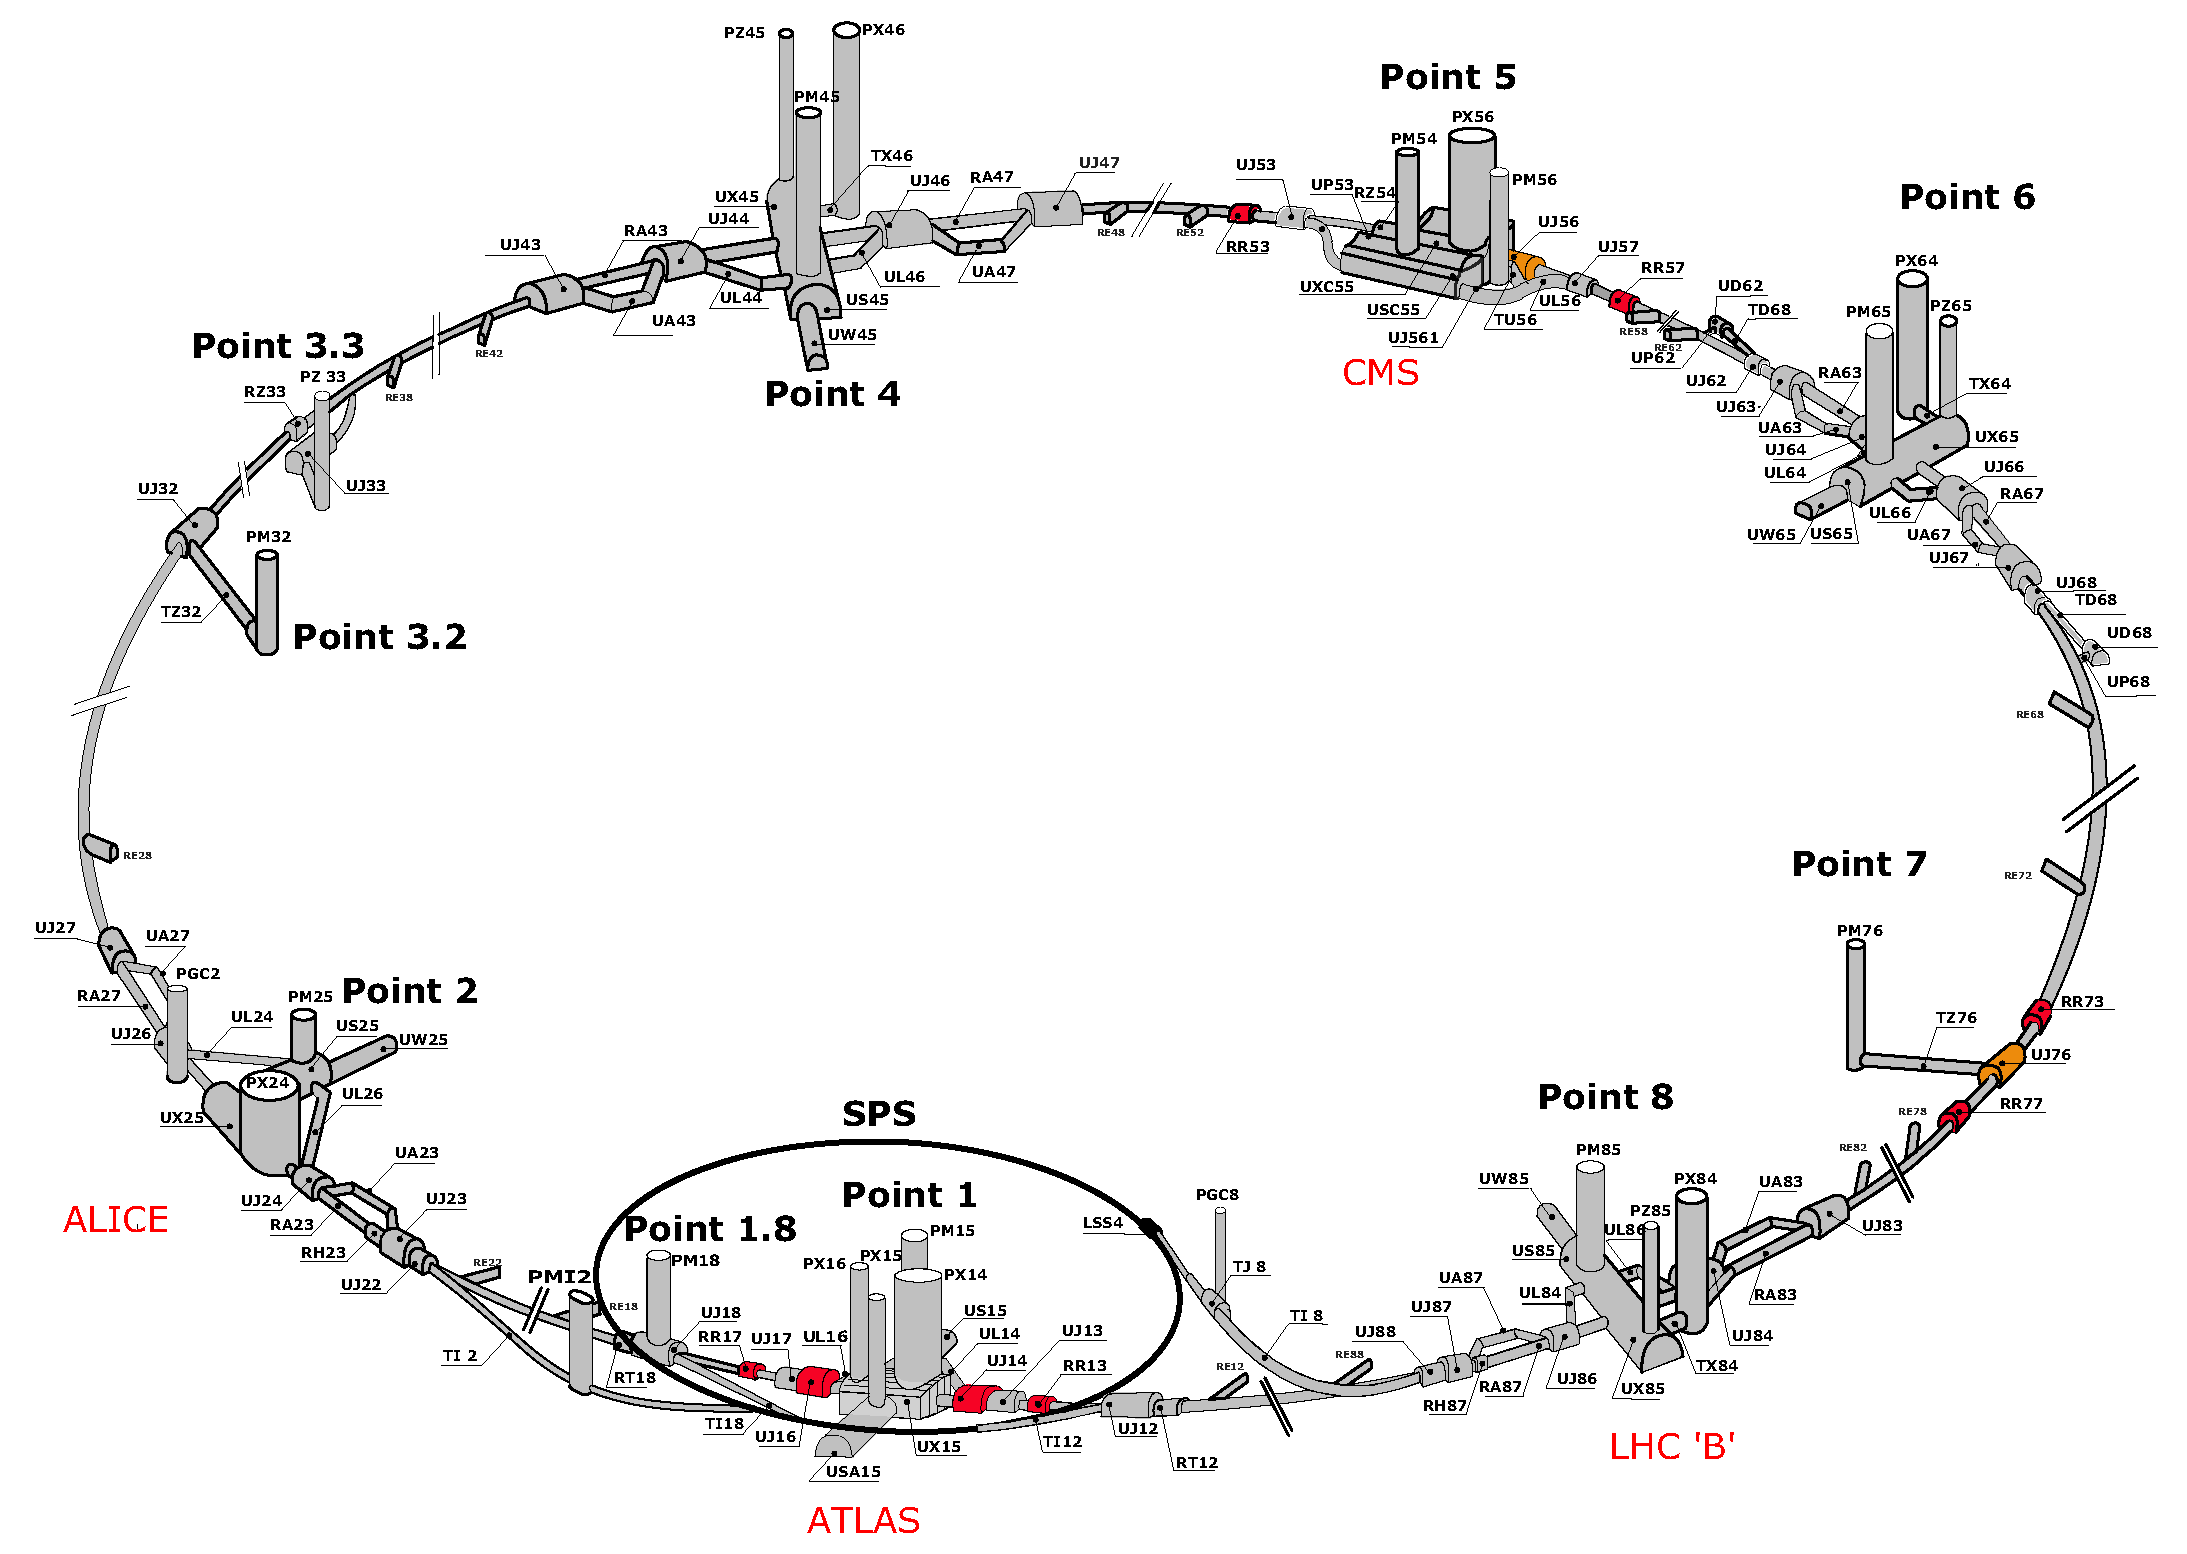
\includegraphics[width=.6\textwidth]{Pictures/LHClayout.PNG}
    \caption{LHC layout \cite{LHCref}}
    \label{fig:LHClayout}
\end{figure}

Superconducting magnets in the LHC main dipoles create a magnetic field of $\approx 8$ T to bend the proton beams into the circlular path of the collider. Figure \ref{fig:dipolemagnet} shows the flux in a dipole cross-section. The opposing direction beamlines are shown centered and the flux is shown to be high (and directionally opposed) in the center of each beam. To maintain these fields, the magnets operate at below 1.9 K. Pressurized superfluid helium chosen for its low visosity and high specific heat cools the dipole magnets. Once the two LHC rings are filled from the SPS, the center-of-mass energy of the beams increases until it reaches peak energy after about 28 minutes. Finally, proton bunches separated by 25 ns collide simultaneously in each detector.  

\begin{figure}[!h]
        \centering
    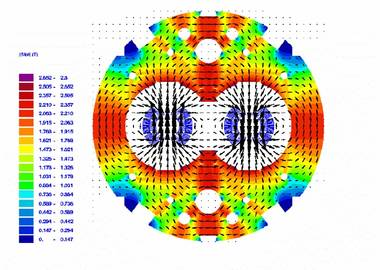
\includegraphics[width=.6\textwidth]{Pictures/dipolemagnet.jpg}
    \caption{ Flux within an LHC dipole cross-section \cite{LHCref}}
    \label{fig:dipolemagnet}
\end{figure}

\section{ATLAS}
The LHC creates proton-proton collisions at the rate and energy necessary for pushing the boundaries of particle physics, but identifying and reconstructing the tracks of such energetic particles is no mean feat. A Toroidal LHC ApparatuS (ATLAS) and the Compact Muon Solenoid (CMS) are multi-purpose detectors built to search for a wide range of particle interactions and the measurement of their properties. Both experiments measured a particle consistent with the Higgs boson in 2012, and their agreement was a key verification of the discovery. The following sections describe each major component of the ATLAS detector, shown in Figure \ref{fig:ATLASdet}, so to highlight their role in the measurement of $H\rightarrow WW \rightarrow \ell\nu\ell\nu$. 

ATLAS utilizes a coordinate system with its origin at the center of the detector (the ``interaction point") and z-axis along the beam pipe. The x-axis points from the interaction point to the center of the LHC ring, and the y-axis points upward. The experiment uses cylindrical coordinates $(r, \phi)$ where $\phi$ is the azimuthal angle around the beam pipe. The pseudorapidity and the transverse momentum are defined in terms of the polar angle $\theta$ as $\eta = -\ln( \tan(\theta/2))$ and $p_T = p\sin\theta$, respectively. 
\begin{figure}[!h]
    \centering
    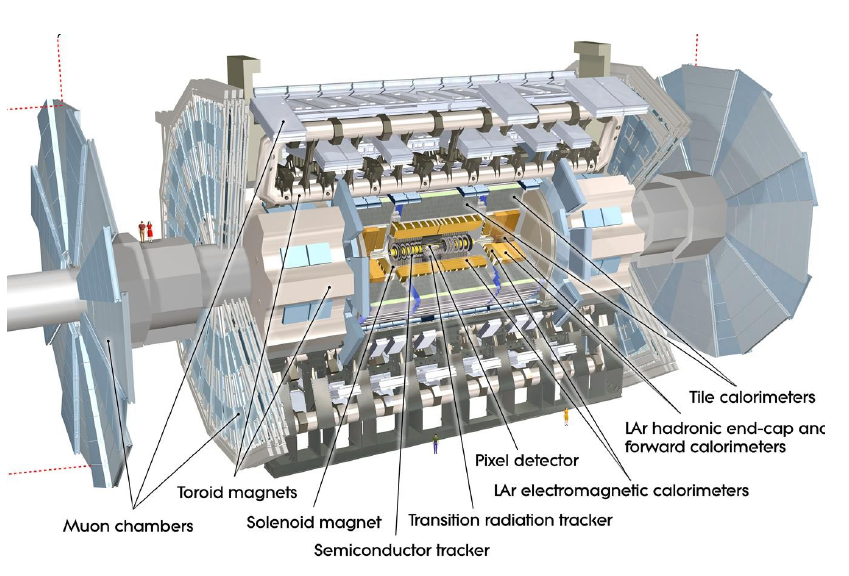
\includegraphics[width=.7\textwidth]{Pictures/ATLASdetector.PNG}
    \caption{Computer-simulated ATLAS detector schematic \cite{detector}}
    \label{fig:ATLASdet}
\end{figure}

The Inner Detector (ID) detects charged particles with $|\eta| < 2.5$ in a 2 T solenoidal field. It consists of $3$ layers of pixel sensors, $4$ layers of silicon strips, and $72$ straw layers of transition radiation tracker modules. The ID describes particles closest to the interaction point and locates track parameters with great resolution due to its high granularity \cite{detector}. 

The ATLAS detector contains 3 superconducting magnet systems---the central solenoid, barrel toroid, and 2 endcap toriods. The central solenoid provides a magnetic field for the inner detector while the toroids create a strong magnetic field for for the muon detector. These magnets were built to create the largest possible uniform magnetic field to maximize the momentum resolution on particle tracks. They also need to use as little material as possible so as to not unduly influence particles in the detector. The toroids in the barrel and endcap each have 8 coils and create a 4 T magnetic field while the central solenoid creates a 2 T magnetic field in the inner detector. Combined the magnet systems contain more than 100 km of superconducting wire which are cooled to working temperatures below 5 K \cite{detector}. 

The Muon Spectrometer (MS) precision chambers provide muon momentum measurements at a high resolution over a wide range of $p_T$. The MS consists of $3$ layers of Monitored Drift Tube chambers covering $|\eta| < 2.7$ and an inner layer of Cathode Strip Chambers with $|\eta| > 2.0$ in the small wheel of the endcap. In addition, it includes trigger chambers that contain $3$ layers of Resistive Plate Chambers ($|\eta| < 1.05$) and $3$ layers of Thin Gap Chambers ($1.05 < |\eta| < 2.4$). As the outermost subdetector, the MS provides precise muon momentum measurements along the muon trajectory, and the muon chambers are located with a precision of under $60$ $\mu$m. The MS also contains a system of three superconducting toroidal magnets each with eight coils providing a magnetic field with a bending integral of up to $6$ Tm \cite{detector}. 

Calorimeters provide detailed information about the energy deposited as particles pass through. Electromagnetic calorimeters detect and halt the motion of electrons and photons while the hadronic do the same for hadrons. Muons and neutrinos are able to pass through the calorimeters to the MS \cite{detector}. 
%The electromagnetic and hadronic liquid Argon and scintillating calorimeters pass information from the location of energy deposits to the various idenfication and reconstruction algorithms \cite{detector}. 

\section{The High-Luminosity LHC and Inner Tracker}
The LHC attained its paramount design goal by discovering the Higgs boson in 2012. Its operation at higher energy and luminosity has led to rigorous measurements of Higgs boson properties as well as searches for new physics beyond the Standard Model. While more data collection is planned in Run 3 starting in 2021, new colliders and detectors take decades to design, develop and build, so the plans for upgrading the current detectors are well underway. The High Luminosity LHC will operate at 14 TeV starting in 2027. The HL-LHC will begin with 5--7 times the luminosity of the LHC and 10 times the design instantaneous luminosity of the LHC, or $12.6\times10^{-34}$ cm$^{-2}$s$^{-1}$. This huge increase in number of collisions requires substantial upgrades to the LHC including new 11--12 T superconducting magnet systems, compact superconducting cavities for beam rotation and phase control, and new technology beam collimation \cite{HLLHCYellow}. 

Just as the LHC had to be re-designed, so do all the experiments to handle the much higher luminosity. The detectors must be built to withstand more radiation, as the increased collision rate also means a high radiation rate, especially closest to the beamline. They also need greater granularity to be able to reconstruct individual tracks with good resolution. Finally, they have to faster to deal with high numbers of collisions occuring in each proton bunch. When there is a large amount of pile-up it becomes difficult to trace which particle tracks come from the same interaction point. Finally, the increased data creates a complex problem for the trigger system, since it must quickly select and store the events that may hold interesting information. 

Detectors for high energy colliders are not built often---expensive and time-consuming to design and test, so they are made to last at least a decade. I had the opportunity to work on ATLAS detector research and development during the 1.5 years I worked at Brookhaven National Laboratory. Though my thesis is not directly related to this work, it was formative and extremely interesting, so I touch on this in the next section. Because I worked on the new ATLAS Inner Detector, termed the Inner Tracker, for the HL-LHC, I discuss this sub-detector and the particular role I played in its assembly in Appendix \ref{sec:ITk}.

